

\section{Self-organizing systems}
\begin{quote}\textit{Cell and tissue, shell and bone, leaf and flower, are so many portions of matter, and it is in obedience to the laws of physics that their particles have been moved, moulded and conformed. They are no exceptions to the rule that God always geometrizes. Their problems of form are in the first instance mathematical problems, their problems of growth are essentially physical problems, and the morphologist is, ipso facto, a student of physical science.--D'Arcy Thompson, On Growth and Form, (1917).} \end{quote}

D'Arcy Thompson's celebrated book  \emph{On Growth and Form} \cite{thompson_1992} is a scientific manifesto rejecting the idea that there is ``something more'' in living matter as compared to inanimate matter (vitalism), and instead argues that the growth and shapes of living organisms are dictated by the laws of physics and should be mathematized. In his view,  honeycomb structure built by bees, the spiral shape of a snail shell, aster-like flowers, or morphological transformations between different species of fish are not an arbitrary results of adaptation by natural selection, but rather strongly constrained by physics. D'Arcy supports these arguments by drawing analogies between shapes observed in living and in inanimate matter. For instance, he argues that the spherical shape of soap bubbles and cells or hexagonal shapes found in honeycomb and corals are governed by the same physical mechanisms. He recognizes that the laws of physics explain the formation of regular patterns of clouds or sand ``by reference to their antecedent phenomena'', i.e.~without a pre-established plan, and argues that growth and form in living systems also results from their ability to organize  according to the laws of physics. Following this argument, he refutes the notion of teleology, according to which the end result would explain a developmental process (``biological structure A forms to enable biological function B''), and rather focuses on causality. More than a hundred years after Thompson's book, his foundational ideas strongly influence the field of physical biology, which largely revolves around the central theme of \emph{self-organization} in life. Although \citet{turing1952} shifted the focus to chemical processes, the field of mechanobiology highlights the interplay between mechanical and chemical aspects of patterning, self-organization and morphogenesis in biology \cite{bois2011,doi:10.1146/annurev-biophys-070816-033602,Burkart:2022tu,Gross:2019ug}.



\begin{figure}
	\centering
	\includegraphics[width=\textwidth]{fig1.pdf}
		\caption{\label{fig_1_1} (a) Self-organization of wave-generated cusps on shorelines  \cite{coco2007} (top),  wind-generated  sand ripples \cite{anderson1990} (bottom).  (b)  Bifurcation diagram representing self-organization of supra-cellular actin rings above a threshold activity (reproduced from \cite{hannezo2015}). (c)  Skin patterns in animals can be explained by Turing instabilities based on an activator-inhibitor model \cite{turing1952}.}
\end{figure}

Self-organization is defined as a spontaneous formation of an organized structure at a global level through interaction between building blocks at the local level. This emergent behavior is an inherent characteristic of driven systems that exist far from thermodynamic equilibrium. %Systems are in thermodynamic equilibrium when there is no net flow of matter or energy, either within the system or in the surrounding. 
When a passive systems evolves towards its equilibrium state, entropy increases and energy is dissipated until equilibrium is reached, and then all fluxes are zero. By contrast, in  systems driven out-of-equilibrium through exchange of matter and/or energy with the surroundings, steady-states are possible with high entropy and sustained dissipation and fluxes \cite{chung2022,prigogine1963,nicolis1977}.  Energy input enables the self-organization into states with spatio-temporal order. Such self-organization in driven systems is ubiquitous across different scales, including the self-organization of ocean circulation \cite{Michael2017}, the formation of  coastlines and sand ripples under the action of waves and wind \cite{coco2007,anderson1990}, Fig.~\ref{fig_1_1}(a), or the active maintenance of membrane-less organelles by liquid-liquid phase separation within cells \cite{hyman2014}. Living systems are in general driven out-of-equilibrium by metabolism, and in particular through the transformation of chemical energy into mechanical work. This process that can be understood using the physical framework of \emph{active matter} \cite{marchetti2013}. To highlight the fundamental features of pattern formation in active matter, we describe next a minimal model for the actin cytoskeleton. Furthermore, this prototypical model provides a gentle introduction to actin dynamics and is a background for the new models proposed in this Thesis.

\section{The actin cytoskeleton and its active self organization}

The actin cytoskeleton is an inherently active  sub-cellular system consisting of a polymeric network of actin filaments and binding proteins. The continuous assembly and disassembly of this network, within turnover times of about 10s, and the binding/unbinding of cross-linkers and myosin motors consume energy from hydrolysis of ATP. As a consequence, the network behaves like an active viscoelastic fluid. Active gel theories are hydrodynamical models that have contributed to the understanding of how activity leads to emergent self-organization \cite{Prost:2015aa}. A mechanism by which active gels form out-of-equilibrium patterns is through self-reinforcing flows, during which a region of higher density of cytoskeletal material becomes locally more contractile, and hence generates a flow towards this region, which further reinforces the higher gel density and triggers a positive feedback loop. The interplay between gel viscosity, friction  with a substrate, turnover and diffusion of cytoskeletal components determines the critical activity for pattern formation and the typical spacing between foci of high density, Fig.~\ref{fig_1_1}(b). This conceptual framework has been mapped into a minimal 1D active gel model, which we describe next, and used to understand the assembly of actomyosin supra-cellular rings \cite{hannezo2015}.



In this model, balance of linear momentum in the gel is expressed along the  $x$  coordinate as
\begin{align}
	& \eta \frac{\partial^2 v}{\partial x^2} +   \frac{\partial \lambda(\rho)}{\partial x}   = \gamma  v,  \label{eq_1}
\end{align}
where the first term is the force density from viscous stresses with $\eta$ the gel viscosity and $v$ the velocity, the second is the force density from  the active contractile stress, which depends on density  $\rho$, and the last one is a frictional force density with coefficient $\gamma$.
This equation is coupled to a partial differential equation encoding mass conservation in the gel
\begin{align}
	& \frac{\partial \rho}{\partial t} + \frac{\partial (\rho v)}{\partial x}  -D \frac{\partial^2 \rho}{\partial x^2} - k(\rho-\rho_0)=0, \label{eq_2}
\end{align}
which states that local changes of gel density are caused by advective and diffusive transport, with diffusivity $D$, and by polymerization and depolymerization, where $k$ is the rate constant and $\rho_0$ the steady-state density for a uniform gel \cite{hannezo2015}. Linear stability of this model shows that beyond a critical activity, the uniform and quiescent steady state given by $v(x,t)=0$ and $\rho(x,t) = \rho_0$ becomes unstable and the system self-organizes into a dynamical steady state with foci of self-reinforcing flows.

We highlight next a number of features of this prototypical active gel model.\begin{enumerate}
	\item Nonlinearity. Nonlinearity makes it possible for the system to exhibit multiple solutions or to break symmetry. {In developmental biology, this nonlinearity provides resistance to perturbation or phenotypic robustness} \cite{green2017}. For instance, the self-assembly of supra-cellular rings described by Eqs.~(\ref{eq_1}) and~(\ref{eq_2}) results in high density regions, whose exponential densification as predicted by the linearized analysis is stabilized by nonlinearity.

	\item Bifurcation, i.e, a sudden change in qualitative behavior, number or/and stability of steady states, upon smooth variation in the model parameters.
	\item Pattern formation through a positive or negative feedback loop.
	The loss of stability of a uniform of high symmetry state is marked by symmetry breaking, leading to spatially inhomogenous patterns with a regular wavelength such as the actin foci predicted from Eqs.~(\ref{eq_1}) and~(\ref{eq_2}). These instabilities are driven by the self-reinforcing flows that result from a positive feedback between density and flow. This self-enhancing buildup of density is controlled by negative feedbacks between density and turnover and between density gradients and diffusion. Notable examples of self-organization from positive and negative feedback dynamics are hexagonal and stripy patterns appearing in the skin of animals Fig.~\ref{fig_1_1}(c), which  can be  described by the system of reaction-diffusion equations put forth by  \citet{turing1952}. The simplest Turing model that supports patterning comprises two species  $u$ and $v$, governed by
	\begin{align}
		& \frac{\partial u}{\partial t} =f(u,v) +D_u \frac{\partial^2 u}{\partial x^2},  \\ &
		\frac{\partial v}{\partial t}=g(u)  - k_v v + D_v \frac{\partial^2 v}{\partial x^2}.  \nonumber
	\end{align}
	Species $u$ promotes the production of  substance $u$ as well as substance $v$ through functions $f$ and $g$. However, substance $v$ inhibits the production of both substance $v$ and $u$ due to self-inhibition through $k_v$ and function $f$. Classic Turing instabilities appear when the ratio $D_v/D_u$ of the two diffusion constants increases beyond a threshold. This condition breaks the stability of a uniform state and spontaneously bifurcates to alternating  waves of concentration differences for $u$. Here, the feedback loops provide the generic mechanism for self-organization. Positive feedback through functions $f$ and $g$ leads to the amplification of perturbations and negative feedback triggers a response that controls the growth of a perturbation.
\end{enumerate}

\section{Self-organization of sub-cellular cytoskeletal networks}

Biological structures across length-scales, from the molecular to the organ level, adopt their shape and composition through the self-organization of patterns \cite{isaeva2012,sekimura2013}, which need to balance robustness and adaptability. Focusing on cytoskeletal networks, in this section we review the organization of actin filament networks at sub-cellular scales, and how reconstituted systems recapitulate these network architectures suggesting a central role of self-organization. We also briefly discuss self-organization in microtubule and intermediate filament networks.


\subsection{The actin cytoskeleton}

The actin cytoskeleton is a crosslinked and dynamical network of actin filaments. It is composed of more than $100$ structural and regulatory proteins  \cite{kelkar2020, chugh2018, thomas2012} such as myosin-II, fascins, $\alpha$-actinin, ADF/cofilin, and profilin. This network is inherently out-of-equilibrium, i.e.~exposed to a continuous flux of energy from  Adenosine triphosphate (ATP) hydrolysis. As a consequence, actin-binding proteins such as myosin-II, fascins or $\alpha$-actinin attach to actin filaments, possibly slide along them, and exert contractile stress through complementary microscopic mechanisms \cite{murrell2015, lenz2012, koenderink2018}. Moreover, proteins such as ADF/cofilins and profilin actively regulate actin filament disassembly  and polymerization \cite{rosenblatt1997, murrell2015,krishnan2009}, and hence, even if these processes balance, the resulting steady-state is highly out-of-equilibrium. From a mechanical standpoint, the actin cytoskeleton exhibits a diversity of behaviors. Depending on the relative importance of different active molecular mechanisms within the network and its architecture, actin gels can either push by polymerization-induced forces or pull by contractile forces induced by myosin motors, cross-linkers or depolymerization. Depending on the rate of deformation compared to the turnover timescale of its constituents, it can either store elastic energy or dissipate it like a fluid \cite{kollmannsberger2011}.

This complex interplay of molecular, biochemical and mechanical processes allows the cortical network to self-organize into a variety of architectures, each  playing different biological roles. Because actin filaments are polar, these network architectures can be classified depending on their orientational order as reviewed next.


\subsubsection{Isotropic actin networks}

In  suspended cells, on a soft substrate or in membrane blebs, the actin cortex adopts an isotropic and relatively sparse architecture \cite{morone2006, svitkina2020}, Fig.~\ref{chap_1_fig_1}(a). The isotropy of the network can be explained by several mechanisms including thermal vibrations that tend to randomize the network \cite{salbreux2009,anne2016}, actin turnover and severing tending to destabilize any degree of anisotropy in the network, and actin polymerization lacking any preferential orientation \cite{svitkina2020}. In cells spread on stiff surfaces, isotropic actin networks coexist  with other architectures described below. The isotropic architecture leads to isotropic network tension, which contributes to cell rounding at the onset of mitosis \cite{salbreux2012, kelkar2020}.


\begin{figure}
	\centering
	\includegraphics[width=0.98\textwidth]{fig2.pdf}
	\caption{\label{chap_1_fig_1} Diverse architectures in the actin cytoskeleton. (a) Isotropic network in the actin cortex of a spherical cell \cite{kelkar2020}. (b) Polar sheets (lamellipodia) and spikes (fillipodia) at the edge of an adherent cell \cite{Mejillano:2004wx}. (c)  Nematic actin bundles (i) during cytokinesis \cite{anne2016}, (ii) during supra-cellular wound healing \cite{10.1242/jcs.109066}, (iii) forming patterns of stress fibers in adherent cells \cite{hotulainen2006}, or (iv) during actomyosin-dependent cellularization \cite{dudin2019}. (d) Actin clusters with star or aster architecture reproduced from  \cite{xia2019} in (i) and from \cite{fritzsche2017} in (ii).% (ii) reconstituted systems \cite{murrell2012} and (iii) tactoids in a reconstituted system \cite{weirich2019}.  
	(e) Topological defects of actin orientation in an adherent cell \cite{schakenraad2020}. }
\end{figure}

\subsubsection{Polar sheets and spikes}

Adherent cells often exhibit at their edge a branched actin network sheet called lamellipodium. Spike-like protrusions of bundled actin filaments such as filopodia are also common at cell edges. These sheets and spikes are polar, Fig.~\ref{chap_1_fig_1}(b), with  plus ends pointing towards the cell edge, push on the plasma membrane thanks to polymerization-induced forces, and enable cells to migrate and probe their environment. Filopodia grow depending on actin polymerases  VASP and formins \cite{svitkina2003} and are rich in crosslinkers \cite{bartles2000}, whereas actin polymerization in lamellipodia is primarily controlled by Arp2/3. Filopodia and lamellipodia are devoid of myosin-II and hence are non-contractile \cite{nemethova2008}. The lamellipodium progressively looses its polarity as the network moves backward in the cell during retrograde flow \cite{svitkina2020}. Likewise, polar filopodial bundles are recycled into nematic contractile bundles, reviewed next, during retrograde flow \cite{nemethova2008,doi:10.1091/mbc.e08-01-0034}.


\subsubsection{Nematic actin bundles}

Nematic actin bundles are dense elongated structures where actin filaments are aligned along their axis in a bipolar configuration, i.e.~on average there is an equal number of filaments pointing with plus and minus ends in either direction along the axis. These structures assemble in a variety of cellular contexts, including cytokinesis \cite{anne2016}, wound healing at sub-cellular 
\cite{mandato2001} and supra-cellular scales \cite{10.1242/jcs.109066}, stress fibers \cite{hotulainen2006}, or during actomyosin-dependent cellularization \cite{dudin2019}, Fig.~\ref{chap_1_fig_1}(c). 

Actin binding proteins such as $\alpha$-actinin  and myosin-II contribute to the tight packing of actin filaments into nematic bundles \cite{blanchoin2014,winkelman2016,lehtimaki2021, laporte2012}. As bundles emerge,  crosslinkers may bind at a higher rate due to favorable filament orientation  \cite{courson2010}. Additionally, the presence  and amount of crosslinkers slows down turnover \cite{SCHMOLLER2011350}  stabilizing dense and cross-linked actin structures. The higher density allows more cross-linkers to bind to the network,  further stabilizing the bundle architecture through positive feedback. The higher cytoskeletal density in nematic bundles and the increased ability of myosin-II to contract an aligned network leads to high, localized and anisotropic active tension \cite{bergert2015, turlier2014, mayer2010, kelkar2020}. Moreover, binding proteins may locally enhance  orientational order of the actin network  \cite{lehtimaki2021}, which in turn also enhances  contractility \cite{kelkar2020}. Thus, the local orientation of the actin filaments in the network is a major determinant of its active mechanical properties. In rounded cells, a tension inhomogeneity  can lead to the self-organization of a contractile  ring, which divides a cell \cite{greenspan1978, mietke2019_2, mietke2019, koyama2012,gladilin2015,biron2005,turlier2014,sain2015,zhao2016,akkacs1980,poirier2012} or heals a wound in an egg cell \cite{mandato2001}.


\begin{figure}
	\centering
	\includegraphics[width=0.98\textwidth]{fig22.pdf}
	\caption{\label{chap_1_fig_22} Dense nematic actin bundles in adherent cells. (a) Families of stress fibers and association to adhesion complexes \cite{hotulainen2006}. (b) Dynamical reconfigurations of stress fibers near the leading edge \cite{tojkander2015}. (c) Coexistence of nematic bundles and asters. Images taken from  \cite{jalal2019} in (i) and  from \cite{xia2019} in (ii). (d) Geometrically regular organization of stress fibers through adhesion patterning in (i) polar \cite{10.1242/jcs.236604} and (ii) circular \cite{jalal2019} geometries. }
\end{figure}



When placed on a stiff substrate, rounded cells break symmetry as they spread \cite{gupta2015, rens2020,callan2008}.
In such spread cells, contractile actin bundles emerge and often form patterns with regular spacing \cite{jalal2019}. These fibers often interact with the extracellular matrix through mechanosensitive focal adhesions, Fig.~\ref{chap_1_fig_22}(a), which transmit tractions to the extracellular matrix \cite{tojkander2012,livne2016}, thereby enabling spreading and migration. Based on their sub-cellular localization and interactions
with extracellular matrix, nematic bundles of adherent cells are  classified into three families \cite{lehtimaki2021, tee2015, tojkander2015,wirshing2017, yolland2019, jalal2019}, Fig.~\ref{chap_1_fig_22}(a). (i) Dorsal stress fibers are attached to the substrate via focal adhesions and are oriented in a radial direction towards the nucleus. Formins mediate the formation of these fibers, which are devoid of myosin and $\alpha$-actinin, and are thought to be non-contractile \cite{lehtimaki2021}. (ii) Transverse stress fibers are oriented along the cell edge and perpendicular to dorsal fibers. They are not connected to the extracellular matrix via focal adhesions and are decorated with both $\alpha$-actinin and myosin. (iii) Ventral stress fibers are generated through the coalescence of pre-existing radial and transverse stress fibers, are contractile,  and are connected to focal adhesions at both ends.

Stress fibers are highly dynamical, with frequent nucleation and fusion events near the leading edge, Fig.~\ref{chap_1_fig_22}(b). Ventral stress fibers assemble through a fusion of radial and transverse arches. However, the mechanism leading to the formation of dorsal and transverse fibers is still an open question. It is unclear to what degree stress fibers emerge from the recycling of pre-existing structures, such as filopodia \cite{nemethova2008,doi:10.1091/mbc.e08-01-0034} or focal adhesions, or assemble de novo. Observations in cells,  reconstituted systems and simulations suggest that stress fibers can assemble from the actin cortex without the involvement of stress fiber precursors or actin polymerization at focal adhesions \cite{lehtimaki2021,livne2016,deshpande2015,freedman2018}. In the absence of anchorage sites, straight actomyosin bundles have been observed to self-organize and dynamically fuse with adjacent bundles \cite{lehtimaki2021,livne2016,wirshing2017}. Furthermore, these bundles coexist in a mechanical continuum with a sparse and isotropic actin network  \cite{vignaud2021}. They can also coexist with actin asters to form networks of nematic bundles connecting dense clusters \cite{jalal2019,xia2019}, Fig.~\ref{chap_1_fig_22}(c). By controlling the shape of adhesive cells through adhesion patterning, stress fibers adopt remarkably regular arrangements that depend on cell shape, size, substrate stiffness and degree of maturation \cite{10.1242/jcs.236604,jalal2019}, Fig.~\ref{chap_1_fig_22}(d). 


\subsubsection{Actin clusters}

Actin networks can also form patterns of high-density foci surrounded by convergent filaments in so-called \emph{asters}, \emph{stars} or \emph{foci} \cite{nishikawa2017,xia2019,fritzsche2017}, see Fig.~\ref{chap_1_fig_1}(d). Such high-density punctuated structures naturally emerge in discrete network simulations of the actin cytoskeleton, which establish their emergence and morphology  depending on model parameters such as filament bending rigidity and length,  concentration of motors and crosslinkers, and actin turnover \cite{freedman2018,li2017,yu2018,mak2016, hiraiwa2016, miller2018}. An interplay between  Arp2/3, formin, and capping proteins has also been shown control cluster patterning \cite{xia2019}. Asters can be polarity sorted or have mixed polarity. Simulations predict mixed-polarity asters at intermediate myosin concentration and high cross-linker concentration \cite{freedman2018}, consistent with mixed polarity asters in cells with low myosin-II expression \cite{xia2019}. Actin clusters can be stable  or short-lived \cite{hiraiwa2016,mcfadden2017}. The short lifetime of asters is attributed to fast turnover, de-branching, or filament severing \cite{yu2018,li2017,mak2016}. As mentioned above, nematic bundles can converge into actin clusters to form complex actin organizations, Fig.~\ref{chap_1_fig_22}(c).

\subsubsection{Topological defects}

Orientational order can smoothly vary or develop orientational  \emph{defects}. In nematic systems, these defects have either half-integer charge such as comet-like ($+1/2$) or trefoil-like ($-1/2$), or full-integer charge such as $+1$ spiral-like or $+1$ aster-like defects.  Activity renders $+1/2$ defects motile along their axis of symmetry, whereas due to their three-fold symmetry,  $-1/2$ defects do not propel \cite{thijssen2020,vafa2020}. Topological defects in stress fiber organization have been reported in adherent single cells  \cite{schakenraad2020},  Fig.~\ref{chap_1_fig_1}(e).


\subsubsection{Interplay between actin architectures cellular shape}

Each actomyosin architecture correlates with distinct cell shape deformations. Polar actin bundles form narrow protrusions such as filopodia at the cell periphery, whereas lamellipodial polar networks form sheets \cite{blanchoin2014}. Equatorial actin nematic bundles constrict  dividing cells in the cytokinetic furrow \cite{anne2016}. Nematic defects  facilitate the reorganization of stress fibers supporting cellular shape changes \cite{schakenraad2020}. The role of actin clusters in cell shape deformation has not been systematically analyzed. A more comprehensive review of shape changes driven by nematic architectures is provided in Chapter~\ref{chap_6}.



\subsubsection{Recapitulation of actin architectures in reconstituted systems}

Supporting the idea of self-organization in the actin cytoskeleton, in vitro reconstituted systems mixing actin filaments with cross-linkers or myosin-II motors in different conditions have recapitulated actin architectures observed in cells. Actin filaments and bundling agents alone can produce remarkably regular networks of dense actin bundles  \cite{huber20152}, Fig.~\ref{chap_1_fig_222}(a). Addition of myosin-II motors to actin gels can lead to regular patterns of asters connected by bundles \cite{murrell2012,seara2018}, Fig.~\ref{chap_1_fig_222}(b), or to gels populated by motile nematic half-integer defects \cite{kumar2018,seara2018}, Fig.~\ref{chap_1_fig_222}(c). In a different regime, a suspension of actin filaments and crosslinkers organizes into spindle-shaped clusters of high density and alignment called tactoids \cite{weirich2017}, which can deform and split upon the action of myosin-II \cite{weirich2019}, Fig.~\ref{chap_1_fig_222}(d). By patterning actin polymerization, constricting actomyosin rings have been reconstituted in vitro  \cite{Ennomani2016}, Fig.~\ref{chap_1_fig_222}(e). Finally, cross-linking of actin filaments confined to a lipid vesicle self-organize into bundled rings, which upon addition of myosin-II become contractile and deform the vesicle \cite{bashirzadeh2022, litschel2021}, Fig.~\ref{chap_1_fig_222}(f).


\subsubsection{Actin bundles as templates during development}

Besides their intrinsic functionality, the ability of actin networks to develop patterns of dense bundles can serve as templates during morphogenesis of other structures. One instance is the formation of ridges in butterfly wing scales, which control their optical properties, \cite{DINWIDDIE2014404} and Fig.~\ref{chap_1_fig_777}(a). Mature scales result from the cuticle of dead cells. During development in the wing epithelium, an actin pre-pattern consisting of parallel dense bundle along elongated cellular extensions develops on an homogeneous cell surface, which then guides cuticle deposition and patterning, and is finally disassembled leaving cuticle ridges behind, Fig.~\ref{chap_1_fig_777}(b). Hence, actin patterning plays a guiding role during morphogenesis, but the final functional structure does not contain actin.   

Another remarkable pattern formed by dense and elongated actin structures are the so-called actin microridges. Microridges form in the apical surfaces of mucosal epithelial cells, as shown for scale epidermal cells in different fish species in Fig.~\ref{chap_1_fig_777}(c) \cite{https://doi.org/10.1002/ar.23965}. These maze-like structures form from point-like actin foci, which elongate, reorganize Fig.~\ref{chap_1_fig_777}(d), and eventually protrude out of the apical plane. Their development and maturation is complex, not fully understood and involves myosin contractility, actin crosslinking, and arp2/3 polymerization. The identification of dense actin bundles below the protrusions \cite{BEREITERHAHN1979316} suggests that microridges protrude by a branched network polymerized by arp2/3 out of a pre-pattern of dense nematic bundles organized from the initially isotropic and uniform apical cortex. The initial stages of microridge formation are highly dynamical and can be guided by mechanical cues such as cell stretching, Fig.~\ref{chap_1_fig_777}(d) \cite{10.1083/jcb.201904144}. Although the function of actin microridges remains open, recent work suggests a role as a pre-pattern and structural anchoring for motile cilia \cite{Yasunaga:2022uh}. 


\begin{figure}
	\centering
	\includegraphics[width=0.99\textwidth]{fig222.pdf}
	\caption{\label{chap_1_fig_222} Architectures in reconstituted actin gels. (a) Diversity of regular network organizations in actin filament preparations upon unspecific bundling by crowding agents \cite{huber20152}. (b) Aster and bundle formation in cross-linked actin gels following addition of myosin-II \cite{murrell2012}. (c) Motile nematic defects in actomyosin gels \cite{seara2018}. (d) Formation of tactoids (nematic actin droplets) in (i) cross-linked actin gels \cite{weirich2017}, and (ii) deformation of tactoids by myosin-II activity \cite{weirich2019}. (e) Reconstituted contractile actomyosin ring \cite{Ennomani2016}. (f) Reconstituted actin rings on lipid vesicles with different cross-linkers, which can become contractile upon addition of myosin-II  \cite{litschel2021}.}
\end{figure}


\begin{figure}
	\centering
	\includegraphics[width=0.99\textwidth]{actin_morphogenesis.pdf}
	\caption{\label{chap_1_fig_777} (a) Multiscale organization of the butterfly wing. Ridges in the scales are the result of the cuticle of dead cells formed from the developing wing epithelium. (b) Developmental stages starting form a pre-pattern consisting of dense parallel actin bundles, which guides the patterned deposition of the cuticle, which remains in place once the actin pre-template has disassembled \cite{DINWIDDIE2014404}.  (c) Actin microridges at the apical surfaces of scale epidermal cells in fish \cite{https://doi.org/10.1002/ar.23965} . (d) Formation of actin microridges (top) and biasing of ridge orientation by cell stretch (bottom) \cite{10.1083/jcb.201904144}. (e) Ridge-like structures template and anchor motile cilia \cite{Yasunaga:2022uh}.}
\end{figure}

\clearpage

\subsection{Microtubule networks}

Microtubules are stiff and polar cytoskeletal filaments undergoing turnover. They also form major cytoskeletal networks, which  contribute to cell shape and polarity, and support cell division and chromosome segregation through the assembly of the  spindle apparatus, Fig.~\ref{chap_1_fig_3}(a). The association of microtubules with molecular motors such as kinesins results in an extensile active gel capable of self-organization. Within cells, the physical mechanisms of the active self-organization of the spindle are becoming increasingly clear \cite{Dalton:2022wg}. Reconstituted gels of microtubules and kinesins exhibit a variety of self-organized network architectures, including patterns of asters and vortices \cite{ndlec1997, surrey2001}, Fig.~\ref{chap_1_fig_3}(b). Moreover, dense confined networks of microtubules develop persistent flows driven by the sustained nucleation, motion and annihilation of half-integer defects \cite{sanchez2012}, Fig.~\ref{chap_1_fig_3}(c). Biologically, such sustained active flows are though to drive cytoplasmic streaming \cite{serbus2005}. On a deflated vesicle, half-integer defects formed by a dense extract of microtubules and kinesins interact with the topological confinement of the closed surface to produce local geometric features of high curvature \cite{keber2014}.

\begin{figure}[hb]
	\centering
	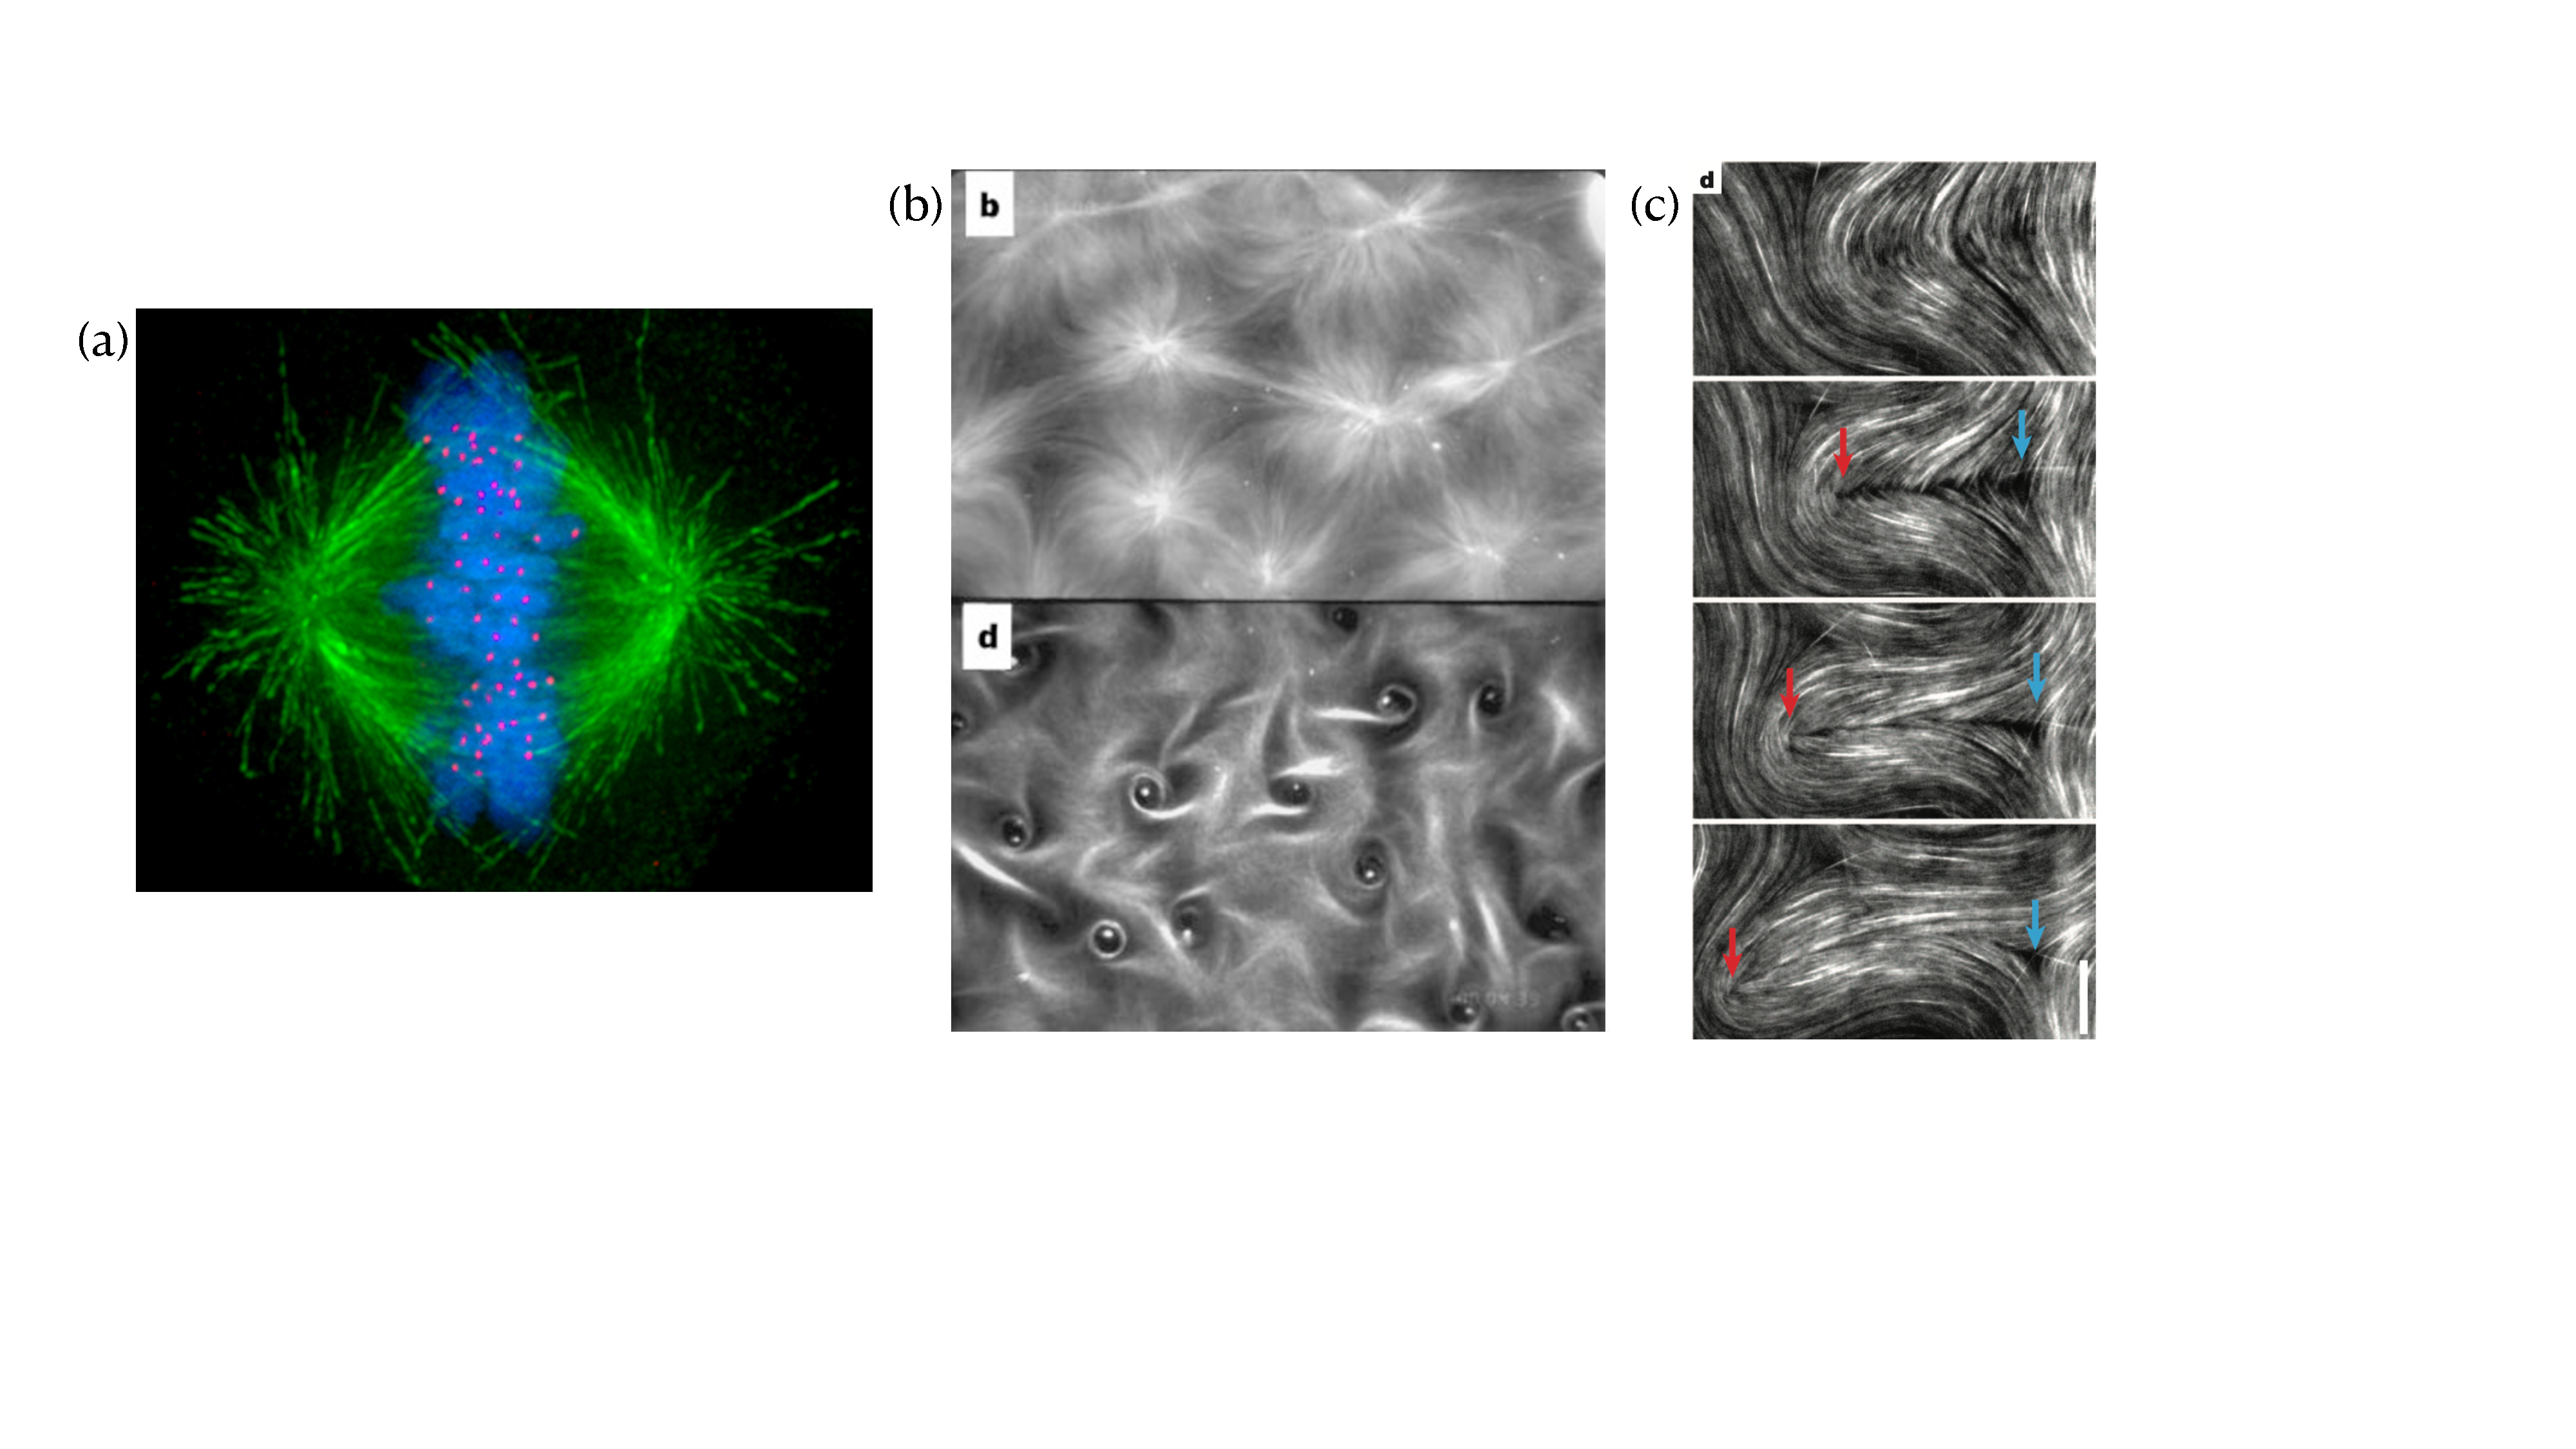
\includegraphics[width=0.9\textwidth]{fig3.pdf}
	\caption{ \label{chap_1_fig_3} Self-organized architectures in microtubule networks. (a) Spindle apparatus during cell division (Wikipedia). (b) Patterns of asters and vortices in reconstituted microtubule-kinesin gels \cite{ndlec1997}. (c) Nucleation and motion of half-integer defects in dense microtubule-kinesin gels \cite{sanchez2012}.}
\end{figure}

\subsection{Intermediate filament networks}

Intermediate filaments (IFs) are another primary component of the cytoskeleton. These filaments are significantly more bendable than actin filaments and microtubules, longer, apolar, and undergo slow turnover \cite{broedersz2014,wagner2007,herrmann2007,godsel2008, lorenz2019}. Individual IFs can further associate into bundles through a balance of electrostatic and hydrophobic interactions \cite{haimov2020}. Although the IF molecular makeup differs widely across cell types, their hierarchical structure comprising coiled-coiled motifs that can unfold when loaded is largely preserved \cite{lorenz2019}, giving rise to the large extensibility and rate-dependent nonlinear force-elongation behavior of IFs \cite{kreplak2005, kreplak2008, qin2009}. %The force plateau upon elongation during uncoiling and the severe re-stiffening at large deformation, are the basis of the widespread view that IFs provide a ``safety belt'' against fast and large cellular deformations \cite{qin2009, golde2018, fudge2008}. 
The crosstalk between IFs and other cytoskeletal networks is receiving increasing attention \cite{huber2015}.

The self-organization of IF networks, which lack molecular motors or specific cross-linkers, into functional architectures has received relatively little attention. Recent work has shown that upon extreme stretch of epithelial monolayers, the IF network within cells undergoes a massive reorganization resulting in a structurally-optimal star-shaped architecture featuring a central node from which IF bundles radiate perpendicularly to the cell boundaries \cite{latorre2018}. Laser ablation experiments show that these taut radial IF bundles contribute to tissue resistance. Recent theoretical work suggests that this transformation is the result of self-organization controlled by network entanglement \cite{pensalfini2022}.


%\subsection{Self-organization and coexistence of actin-based architectures}
%
%Actin-based invitro or reconstituted systems self-organize diverse actin architecture, some of which coexist with each other.  For cells confined to adhesive islands of various sizes self-organize circular, radial and chiral actin bundles, see \ref{architectures}(a). Radial stress fibers and actin cluster also coexist in cells spread on adhesive substrates \cite{jalal2019} see \ref{architectures}a(right). Actin-based reconstituted systems have shown to  self-organize  a lattice of asters interconnected through actin bundles \cite{huber2015_2, weirich2017, murrell2012}, see fig \ref{architectures}(b,c,d), or form crosslinked nematic tactoid and bundles together in a suspension of actin monomers , see fig \ref{architectures}(e). Lastly, a coordinated assembly of actin bundles in hexagonal lattice drives  cellularization in a unicellular relative of animals.
%
%\begin{figure}
%	\centering
%	\includegraphics[width=0.85\textwidth]{chap_1_fig_new.pdf}
%	\caption{\label{architectures} \textbf{Self-organization and coexistence  of diverse actin-based architectures in cells and reconstituted systems}. Images adapted from (a) \citet{jalal2019} (b) \citet{huber20152} (c) \citet{adamatzky2019} (d) \citet{murrell2012} (e) \citet{weirich2017} (f)  \citet{Dudin2019}. }
%\end{figure}


\section{Theoretical models for emergent nematic cytoskeletal architectures}

The focus of this thesis is on the self-organization of nematic active gels, with an emphasis on actin networks. The self-organization of active nematic systems has been addressed using both discrete and continuous descriptions. In discrete models, \cite{bechinger2016, patelli2019, alaimo2017, ehrig2017,keber2014,khoromskaia2017,ellis2018} active nematic systems are resolved at the scale of individual active units, which are usually modeled as self-propelled Brownian particles. The emergent behavior of the system depends on an interplay of fluctuations, active forces generated by individual units, and  alignment and repulsion interactions. Discrete network simulations to specifically understand actin network show that  even obtaining a steady-state uniform network undergoing turnover and sustaining active tension is challenging \cite{freedman2018,li2017,yu2018,mak2016, hiraiwa2016, miller2018}. In general discrete models cannot access phenomena occurring at large length-scales and over long time-scales, such as those involved in the self-organization of the actin cytoskeleton at the cellular scale. Alternatively, continuum models can access the pertinent  mesoscales in time (minutes) and space (10s of microns) using fewer degrees of freedom after numerical discretization. A number of active nematic continuum models have been proposed \cite{vcopar2019,zhang2020, napoli2020,pearce2020,nestler2018,hemingway2016,metselaar2019}. The constitutive laws in these theories can be based on the underlying microscopic dynamics \cite{patelli2019,bertin2013,peshkov2012,doi:10.1126/science.aao5434,Denk:2020vm}, or on symmetry arguments within the framework of  irreversible thermodynamics \cite{simha2002,hatwalne2004,julicher2018, salbreux2022}.

\subsection{Kinematics}

At large length and time scales, the relevant dynamics of a planar nematic system can be expressed in terms of
\begin{enumerate}
	\item A change in position of material particles represented by flow field $\bm{v}(\bm{x},t)$.
	\item A change in the nematic orientational order of the system, which breaks  isotropic symmetry. At any given time, orientational order can be quantified by a coarse-grained quantity called the nematic order tensor
	\begin{align} \label{5_1}
		q_{ab}  & =  \left\langle m_a m_b - \frac{\delta_{ab}}{2}\right\rangle,
	\end{align}
	where $\bm{m} = \textup{sin}(\theta) \hat{\bm{e}}_1 + \textup{cos}(\theta) \hat{\bm{e}}_2 $ is the orientation of individual molecules and $\langle \cdot  \rangle$ represents the microscopic average of the ensemble \cite{mottram2014}. By definition, the nematic tensor is symmetric and traceless, i.e, $q_{ab}=q_{ba}$  and $q_{aa}=0$. The microscopic representation of the nematic tensor can be described in terms of a probability distribution of orientations $f(\theta)\geq 0$, which must satisfy the normalization condition  $ \int_0^{2\pi} f(\theta)d\theta=1$ and the apolar character of the network, $f(\theta) =f(\theta+\pi)$. In 2D, any symmetric and traceless tensor can be represented as
	\begin{equation}
		q_{ab} = S\left(n_a n_b -\frac{\delta_{ab}}{2}\right),
	\end{equation}
in terms of a scalar $S$ and a unit vector $\bm{n}$. Comparing this expression and Eq.~(\ref{5_1}), we identify $S= 2 \langle (\bm{m} \cdot \bm{n})^2 -1/2 \rangle$ as a measure of deviation of molecular orientation relative to the axis defined by $\bm{n}$, which can be interpreted as the net molecular orientation \cite{selinger2016}.
\end{enumerate}
\subsection{Governing equations}
The dynamics of a prototypical active nematic system follow from the coupled set of  governing equations
\begin{align}
	& \bm{\nabla} \cdot \bm{\sigma} - \bm{\nabla} p = \bm{f},   \label{12_1} \\ &
	\bm{\nabla} \cdot \bm{v} = 0 , \label{11_1}  \\ &
	\frac{d\bm{q}}{dt}  = \bm{s}(\bm{d},\bm{w}) + \frac{1}{\eta_{\rm  rot}}\bm{h},  
\end{align}
where the total stress $\bm{\sigma} = \bm{\sigma}^a + \bm{\sigma}^e + \bm{\sigma}^d$ contains an active component $\bm{\sigma}^a$, a dissipative component $\bm{\sigma}^d$ and a reversible elastic component $\bm{\sigma}^e$,  $\bm{f}$ is an external force density, and the pressure field $p$ is determined using the incompressibility constraint in Eq.~(\ref{11_1}). $d\bm{q}/dt$ is the material time derivative of $\bm{q}$, $\bm{s}$ account for changes in $\bm{q}$ due to fluid rotation and flow-induced alignment, $\eta_{\rm rot}$ is the orientational viscosity and $\bm{h}$ is the variational derivative of a free-energy potential with respect to $\bm{q}$. The free-energy potential encapsulates the equilibrium physics of the nematic system and builds on liquid-crystal theory \cite{de1993,edwards1990,beris1994}.   These governing equations are often solved with numerical algorithms such as Lattice Boltzmann methods \cite{desplat2001, denniston2004,marenduzzo2007,cates2009} or finite element methods \cite{goudiaby2021,becker2008, norton2018}.

\section{Knowledge gap}

One of the motivations to study the self-organization of active nematic gels is that the mechanisms leading to one of the most prominent architecture in the actomyosin cytoskeleton, dense nematic bundles as shown in Figs.~\ref{chap_1_fig_1} and~\ref{chap_1_fig_22}, remain poorly understood and to our knowledge no prior theory explains their mesoscale self-assembly. Previous approaches to active nematic systems have focused on incompressible liquid crystals. However, actin gels are highly porous and exhibit very large density variations controlled by advection of cortical materials, turnover, and diffusion of disassembled constituents. In turn, density controls activity and passive mechanical properties. Hence actin gels cannot be described as incompressible active fluids. Furthermore, in crowded liquid crystals, local alignment is a requirement to densely pack elongated constituents, leading to extended nematic states with defects required by topological constraints. Instead, porous actin networks can exhibit extended isotropic states without defects, and nematic order is presumably induced by flows and by active mechanisms. Finally, little attention has been paid to the formulation of active nematics on deformable surfaces, despite the fact shape and nematic architecture are strongly linked  both in cells and in reconstituted vesicle systems  \cite{anne2016, Dong,mandato2001,weirich2019,keber2014}. Recent exceptions are the theoretical framework by \citet{salbreux2022} and the computational study by \citet{https://doi.org/10.48550/arxiv.2205.06805}. In addition to model formulation, the field lacks a general computational framework capable of solving the multi-field governing equations in their full nonlinearity, including the coupling between in-plane density-dependent active nemato-hydrodynamics and shape. Finally, we lack a unified understanding of actin network polymorphism, and more specifically of the physical mechanisms that enable a single active material to adopt very different network architectures with distinct cellular functions. 


\section{Goals and objectives}

This thesis has two main goals. The first goal is to understand the physical mechanisms that control the active self-organization of the actin cytoskeleton into diverse nematic architectures, focusing on 2D gels representative of a flat actomyosin cortex.  To achieve this goal, we establish the following objectives:
\begin{enumerate}
	\item Develop a thermodynamically consistent mathematical model of an active nematic gel and pertinent to the actin cytoskeleton, in particular accounting for the appropriate mechanisms coupling density, hydrodynamics and nematodynamics.
	\item Develop a numerical framework to approximate the solution of the proposed mathematical model in biologically relevant situations.
	\item Perform a linear stability analysis of the model to map the parameter regions where destabilization of a homogeneous steady state leads to pattern formation.
	\item Perform simulations to study the fully nonlinear behavior of the self-organized patterns in different parametric regimes of the model.
	\item Identify the key parameters that control actin gel polymorphism and dynamics.
	\item Validate key assumptions of the active nematic gel theory using discrete network simulations of the cytoskeleton.
\end{enumerate}
The second goal of the thesis is to explore the spontaneous shape changes in curved active nematic gels resulting from the self-organization of different network architectures. To reach this goal, we establish the following objectives:
\begin{enumerate}
	\item Extend the proposed 2D active nematic gel theory to arbitrarily curved and deformable surfaces in a covariant and thermodynamically consistent manner.
	\item Develop numerical algorithms to solve the active nematic gel theory under the assumption of axisymmetry to efficiently explore relevant morpho-nemato-hydrodynamical processes such as cell division.
	\item Develop general numerical algorithms in 3D to active nematic gel theory on deformable surfaces and apply it to relevant morpho-nemato-hydrodynamical processes.
\end{enumerate}

\section{Thesis outline}

The Thesis is structured as follows. In the first part, we address the  first goal of the thesis in the following sequence
\begin{enumerate}
\item In Chapter~\ref{chap_2}, we first introduce Onsager's variational formalism as an elegant and useful framework to model the dissipative and active dynamics of biological systems. Based on this formalism, we then develop a general theory for density-dependent active nematic gels.
\item In Chapter~\ref{chap_3}, we present a finite element computational framework to numerically solve the governing equations. We then apply the numerical model to explore wound healing mechanisms in actin gels and self-organized flows and patterns of defects in confined colonies of elongated cells.
\item In Chapter~\ref{chap_4}, we test the idea of physical self-organization of actin nematic architectures. To understand the onset of pattern formation, we perform linear stability analysis of the dynamical equations, leading to explicit formulae for the critical activity required to produce out-of-equilibrium patterns consisting of dense nematic structures coexisting with a low-density isotropic network. We then examine the fully nonlinear regime using simulations and identify physical principles controlling the geometry and dynamics of emergent patterns.
Furthermore,  we seek to validate key assumptions in our active nematic  gel theory required for self-organization of dense nematic bundles. For this, we drive out-of-equilibrium an agent-based microscopic model of the actomyosin network to characterize active tension anisotropy and nematic activity.
\end{enumerate}

In the second part, we address the second goal of the thesis in the following sequence
\begin{enumerate}
	\item In Chapter~\ref{chap_6}, we motivate through experimental observations the investigation of shape changes in active nematic surfaces.
\item In Chapter~\ref{chap_7}, we present a  thermodynamically consistent theoretical framework based on Onsager's variational formalism for density-dependent active nematic gels on deformable surfaces.
\item In Chapter~\ref{chap_8}, we present a computational framework to solve the axisymmetric governing equations, which we use to study the self-organized shape changes in actin cortices  during cell division and polarization.
\item In Chapter~\ref{chap_9},  we present a theoretical and computational 3D framework for the coupled nematic and shape dynamics in an inextensible active liquid crystalline surface, and use it to examine the interaction between shape and defects.
\end{enumerate}
Finally, in Chapter~\ref{chap_10}, we summarize our contributions and outline future avenues of research.
